



\begin{frame}{Problemática}
    \begin{itemize} \setlength\itemsep{1em}
        \item Os jogos digitais estão cada vez melhores e exigindo mais
        complexidade, trazendo mais conteúdo;
        \item O tempo para produzir este conteúdo demanda muito esforço de trabalho.
    \end{itemize}
    
    \begin{figure}[H]
        \centering
        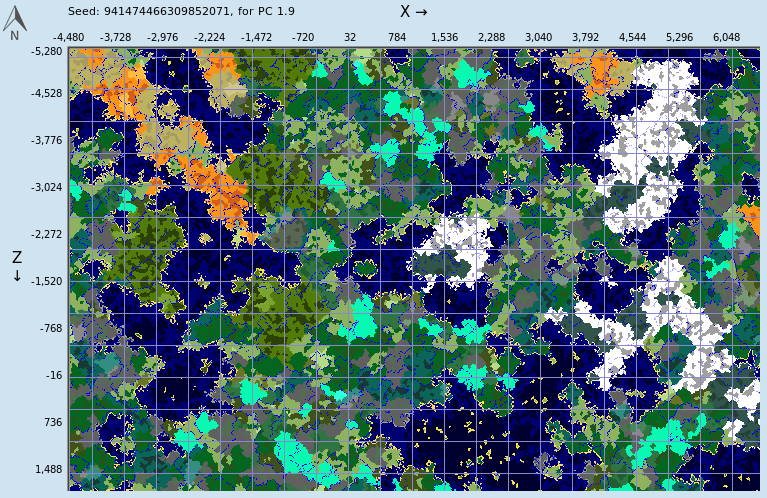
\includegraphics[width=.6\textwidth, height=.5\textheight]{img/chunkbasebiomes}
        \caption{Mapa de biomas de algum mundo do Minecraft.}
        \label{fig:chunkbasebiomes}
    \end{figure}
    
\end{frame}


%\begin{frame}{Introdução}
%    
%\end{frame}

\begin{frame}{Objetivos}
    \begin{itemize}
        \item Objetivo Geral
        \begin{itemize}
            \item Este projeto tem como objetivo gerar mapas de tamanho pseudo-infinitos, com 
            relevo gerado proceduralmente usando ruído 
            de Perlin, de maneira não assistida, os mapas de altura devem representar o 
            relevo de pelo menos dois biomas arbitrários com fronteiras contínuas.
        \end{itemize}
        \item Objetivos Específicos
        \begin{itemize}
            \item Implementar malhas da superfície com tamanho pseudo-infinito;
            \item Selecionar biomas, e as características dos mesmos a ser representadas;
            \item Construir algoritmo para manipular ruído de Perlin e gerar características
                selecionadas do bioma;
            \item Gerar divisões entre biomas sobre a malha de regiões;
            \item Implementar fronteiras contínuas entre biomas;
            \item Comparar resultado com cenários de jogos.
        \end{itemize}
    \end{itemize}
\end{frame}